%% -*- coding: utf-8 -*-
\documentclass[12pt,a4paper]{scrartcl} 
\usepackage[utf8]{inputenc}
\usepackage[english,russian]{babel}
\usepackage{indentfirst}
\usepackage{misccorr}
\usepackage{graphicx}
\usepackage{amsmath}
\usepackage{pgfplots}
\usepackage{listings}
\pgfplotsset{compat=1.9}

\begin{document}
\begin{titlepage}
  \begin{center}
    \large




    \vspace{0.5cm}

    Санкт-Петербургский политехнический университет Петра Великого
    \vspace{0.25cm}
    
    Институт компьютерных наук и технологий
    
    \vspace{0.25cm}
    Высшая школа программной инженерии
    \vfill

    \textsc{Лабораторная работа №4}\\[5mm]
    \bigskip
    {\LARGE Тема: Компилятор GCC. Оптимизация.\\
      Выбор оптимальной опции оптимизации}
  \bigskip
    
    
\end{center}
\vfill

 \newlength{\ML}
\settowidth{\ML}{«\underline{\hspace{0.7cm}}» \underline{\hspace{2cm}}}
\hfill\begin{minipage}{0.5\textwidth}
Работу выполнил студент\\
группы № в13534/22\\
  \underline{\hspace{\ML}} М.\,В.~Андреев\\
  «\underline{\hspace{0.7cm}}» \underline{\hspace{2cm}} 2019 г.
\end{minipage}%
\bigskip
\vfill
 \newlength{\ML}

\settowidth{\ML}{«\underline{\hspace{0.7cm}}» \underline{\hspace{2cm}}}
\hfill\begin{minipage}{0.5\textwidth}
  Работу проверил\\
  \underline{\hspace{\ML}} А.\,В.~Петров\\
  «\underline{\hspace{0.7cm}}» \underline{\hspace{2cm}} 2019 г.
\end{minipage}%
\bigskip
\vfill

\begin{center}
  Санкт-Петербург, 2019 г.
\end{center}
\end{titlepage}
\newpage
\begin{center}
    {\LARGE Постановка задачи}
\end{center}
\par
Цель работы -- выбрать опции оптимизации для приложения.
На основе примера, демонстрирующего различные уровни оптимизации, написать
сценарий, выполняющий следующие действия в цикле:
\begin{itemize}
  \item Компиляцию вашего приложения, не интерактивно обрабатывающего
данные на языке C/C++/Fortran/Objective C/Objective C++/Ada с ключами
оптимизации
\begin{itemize}
  \item -O0
  \item -Os
  \item -O1
  \item -O2
  \item -O3
  \item -O2 -march=native
  \item -O3 -march=native
  \item -O2 -march=native -funroll-loops
  \item -O3 -march=native -funroll-loops
\end{itemize}
\item Вычисление времени выполнения программы (time). Приложение без
оптимизации должно работать по меньшей мере 20 с.
\item Вычисление занимаемого исполняемым файлом дискового пространства (в
байтах) (du).
\end{itemize}

\newpage
\begin{center}
    {\LARGE Ход выполнения работы}
\end{center}
\par
Для нахождения наиболее эффективной опции оптимизации была написана программа
для перемножения двух матриц размером 1000x1000 элементов на языке C.
Исходный код программы приведен в приложении. Время работы исполняемого файла без оптимизации составло 20,44 секунды, что удовлетовряет условию задачи.
\par
Далее был составлен сценарий для компиляции исходной программы и вывода ее времени выполнения в секундах и размера в байтах
Листинг сценария приведен в приложении. Результаты времени исполнения и размера исполняемого файла с использованием разных ключей оптимизации представленны в таблице 1.

\begin{center}
\caption{Таблица 1. Время выполнения программы и ее размер в зависимости от ключа}\\
\begin{tabular}{| l | l | l |}
\hline
Ключ оптимизации & Время исполнения, с & Размер, байт  \\ \hline
-O0 & 20,44 & 8600\\
-Os & 8,42 & 8600\\
-O1 & 9,55 & 8600\\
-O2 & 8,69 & 8600\\
-O3 & 8,39 & 8600\\
-O2 -march=native &	9,31 &	8600\\
-O3 -march=native &	9,75	& 8600\\
-O2 -march=native -funroll-loops &	8,92	& 8600\\
-O3 -march=native -funroll-loops &	8,64	& 8600\\
\hline
\end{tabular}\\
\end{center}
\par
Было выявленно, что исполняемый фаил, скомпилированный с использованием ключа оптимизации -O3, исполняется быстрее всех, вследствие чего он был выбран в качестве оптимальной опции.
\par
Далее была проведена оптимизация с оптимальной опцией и межпроцедурной оптимизацией и оптимизацией времени компоновки (-flto -fipa-*). Результаты времени исполнения и размера исполняемого файла представленны в таблице 2.

\begin{center}
\caption{Таблица 2. Время выполнения программы и ее размер в зависимости от ключа с оптимизацией времени компоновки}
\begin{tabular}{| l | l | l |}
\hline
Ключ оптимизации & Время исполнения, с & Размер, байт  \\ \hline
-O3 -march=native -flto &	8,49 & 8600\\
-O3 -march=native -fipa-reference &	9,94 & 8600\\
\hline
\end{tabular}\\
\end{center}
\par
Было выявленно, что исполняемый файл, скомпилированный с использованием ключа оптимизации -O3 -flto, выполняется дольше на 10 мс.
\par
Далее была проведена оптимизация с оптимальной опцией и с оптимизацией с обратной связью (-fprofile-generate/-fprofile-use). Результаты времени исполнения и размера исполняемого файла представленны в таблице 3.

\begin{center}
\caption{Таблица 3. Время выполнения программы и ее размер в зависимости от ключа с оптимизацией с обратной связью}
\begin{tabular}{| l | l | l |}
\hline
Ключ оптимизации & Время исполнения, сек & Размер, байт  \\ \hline
-O3 -fprofile-generate & 7,83 & 79712\\
-O3 -fprofile-use &	10,18 & 8600\\
\hline
\end{tabular}\\
\end{center}
\par
Было выявленно, что исполняемый файл, скомпилированный с использованием ключа оптимизации -O3 -fprofile-generate, выполняется быстрее всех, однако и его размер существенно больше.
\par
На рисунке 1 представлено соотношение времени работы исполняемого файла в зависимости от ключа оптимизации.
\begin{center}
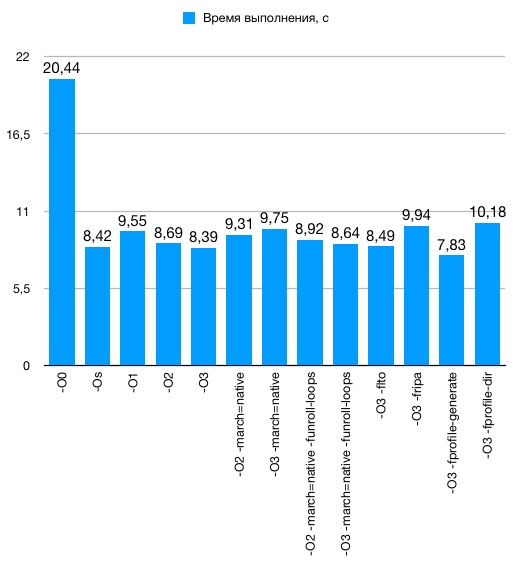
\includegraphics[width=\linewidth]{time.jpg}
\caption{Рисунок 1. Время выполнения исполняемого файла в зависимости от ключа оптимизации}
\end{center}
На рисунке 2 представлено соотношение размера исполняемого файла в зависимости от ключа оптимизации.
\begin{center}
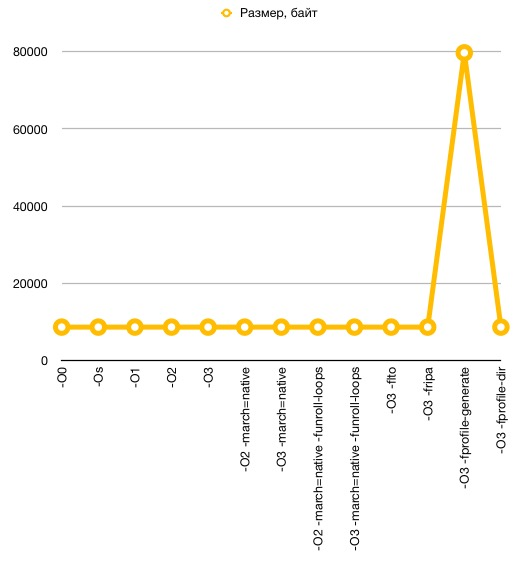
\includegraphics[width=\linewidth]{size.jpg}
\caption{Рисунок 2. Размер исполняемого файла в зависимости от ключа оптимизации.}
\end{center}
\par
\newpage
\begin{center}
    {\LARGE Заключение}
\end{center}
\par
Вывод: в результате выполнения лабораторной работы было выявленно, что размер файла не изменялся до использования оптимизации с обратной связью. Исполняемый файл, скомпилированный с ключом -O3 -fprofile-generate исполнился быстрее (7,83 с), чем исполняемые файлы, скомпилированные с другими ключами, однако его размер был существенно больше. Таким образом, в качестве опимальной была выбрана опция сключом -O3 (Время выполнения файла составило 8,39 с).
\newpage
\begin{center}
    {\LARGE Приложение}
\end{center}

\lstset{ %
language=C,                 % выбор языка для подсветки (здесь это С)
basicstyle=\small\sffamily, % размер и начертание шрифта для подсветки кода
numbers=left,               % где поставить нумерацию строк (слева\справа)
numberstyle=\tiny,           % размер шрифта для номеров строк
stepnumber=1,                   % размер шага между двумя номерами строк
numbersep=5pt,                % как далеко отстоят номера строк от подсвечиваемого кода
backgroundcolor=\color{white}, % цвет фона подсветки - используем \usepackage{color}
showspaces=false,            % показывать или нет пробелы специальными отступами
showstringspaces=false,      % показывать или нет пробелы в строках
showtabs=false,             % показывать или нет табуляцию в строках
frame=single,              % рисовать рамку вокруг кода
tabsize=2,                 % размер табуляции по умолчанию равен 2 пробелам
captionpos=t,              % позиция заголовка вверху [t] или внизу [b] 
breaklines=true,           % автоматически переносить строки (да\нет)
breakatwhitespace=false, % переносить строки только если есть пробел
escapeinside={\%*}{*)}   % если нужно добавить комментарии в коде
}
\begin{lstlisting}[label=code,caption=Произведение матриц]                % Начало блока кода

#include <stdio.h>
#include <stdlib.h>
#include <time.h>

#define N 1000

int main() {
  int **A = (int**)malloc(N * sizeof(int*));
  int **B = (int**)malloc(N * sizeof(int*));
  int **C = (int**)malloc(N * sizeof(int*));

  int i, j, k;

  for(i = 0; i < N; i++) {
    A[i] = (int*)malloc(N * sizeof(int));
    B[i] = (int*)malloc(N * sizeof(int));
    C[i] = (int*)malloc(N * sizeof(int));
  }

  srand(time(NULL));
  for(i = 0; i < N; i++)
    for (j = 0; j < N; j++) {
      A[i][j] = rand() % 10;
      B[i][j] = rand() % 10;
    }

  for(i = 0; i < N; i++)
  for(j = 0; j < N; j++) {
    C[i][j] = 0;
    for(k = 0; k < N; k++)
      C[i][j] += A[i][k] * B[k][j];
    }

  // printf("\nmatrix A\n");
  // for(i = 0; i < N; i++) {
  //   for(j = 0; j < N; j++)
  //     printf("%d ", A[i][j]);
  //   printf("\n");
  // }

  // printf("\nmatrix B\n");
  // for(i = 0; i < N; i++) {
  //   for(j = 0; j < N; j++)
  //     printf("%d ", B[i][j]);
  //   printf("\n");
  // }

  // printf("\nthe result of multiplying\n");
  // for(i = 0; i < N; i++) {
  //   for(j = 0; j < N; j++)
  //     printf("%3d ", C[i][j]);
  //   printf("\n");
  // }

  for(i = 0; i < N; i++) {
    free(A[i]);
    free(B[i]);
    free(C[i]);
  }

  free(A);
  free(B);
  free(C);

  return 0;
}

\end{lstlisting}

\begin{lstlisting}[label=code,caption=Сценарий]
#!/bin/bash

name=$1

gcc -Wall -O0 $1
echo "-O0"
out="$(time ./a.out)"
by="$(du -b a.out)"
echo "byte :$by"

gcc -Wall -Os $1
echo "-Os"
out="$(time ./a.out)"
by="$(du -b a.out)"
echo "byte :$by"

gcc -Wall -O1 $1
echo "-O1"
out="$(time ./a.out)"
by="$(du -b a.out)"
echo "byte :$by"

gcc -Wall -O2 $1
echo "-O2"
out="$(time ./a.out)"
by="$(du -b a.out)"
echo "byte :$by"

gcc -Wall -O3 $1
echo "-O3"
out="$(time ./a.out)"
by="$(du -b a.out)"
echo "byte :$by"

gcc -Wall -O2 -march=native $1
echo "-O2 -march=native"
out="$(time ./a.out)"
by="$(du -b a.out)"
echo "byte :$by"

gcc -Wall -O3 -march=native $1
echo "-O3 -march=native"
out="$(time ./a.out)"
by="$(du -b a.out)"
echo "byte :$by"

gcc -Wall -O2 -march=native -funroll-loops $1
echo "-O2 -march=native -funroll-loops"
out="$(time ./a.out)"
by="$(du -b a.out)"
echo "byte :$by"

gcc -Wall -O3 -march=native -funroll-loops $1
echo "-O3 -march=native -funroll-loops"
out="$(time ./a.out)"
by="$(du -b a.out)"
echo "byte :$by"

gcc -Wall -O2 -march=native -flto $1
out="$(time ./a.out)"
by="$(du -b a.out)"
echo "-O2 -march=native -flto"
echo "byte :$by"

gcc -Wall -O2 -march=native -fipa-reference $1
out="$(time ./a.out)"
by="$(du -b a.out)"
echo "-O2 -march=native -fipa-reference"
echo "byte :$by"

gcc -Wall -O2 -march=native -fprofile-generate $1
out="$(time ./a.out)"
by="$(du -b a.out)"
echo "-O2 -march=native -fprofile-generate"
echo "byte :$by"

gcc -Wall -O2 -march=native -fprofile-use $1
out="$(time ./a.out)"
by="$(du -b a.out)"
echo "-O2 -march=native -fprofile-use"
echo "byte :$by"

gcc -Wall -O2 -march=native -flto -fprofile-use $1
out="$(time ./a.out)"
by="$(du -b a.out)"
echo "-O2 -march=native -flto -fprofile-use"
echo "byte :$by"

gcc -Wall -O2 -march=native -fipa-reference -fprofile-use $1
out="$(time ./a.out)"
by="$(du -b a.out)"
echo "-O2 -march=native -fipa-reference -fprofile-use"
echo "byte :$by"

gcc -Wall -O2 -march=native -flto -fprofile-generate $1
out="$(time ./a.out)"
by="$(du -b a.out)"
echo "-O2 -march=native -flto -fprofile-generate"
echo "byte :$by"

gcc -Wall -O2 -march=native -fipa-reference -fprofile-generate $1
out="$(time ./a.out)"
by="$(du -b a.out)"
echo "-O2 -march=native -fipa-reference -fprofile-generate"
echo "byte :$by"
\end{lstlisting}

\end{document}
